\section{Introduction}
%背景
Large Language Models \citep{gpt,clip,gemini,deepseek,llama3,qwen3} have achieved significant success across various domains and demonstrated exceptional abilities for processing long-context tasks, such as contextual question answering and document summarization \citep{sumsurvey,deepseek_coder,comprehensive}. A key enabler of efficient inference is the KV cache mechanism, which significantly accelerates autoregressive decoding by reducing the computational complexity of self-attention from $\mathcal{O}(n^2)$ to $\mathcal{O}(n)$. However, with the growth of context length, the memory footprint of KV cache and the high computational overhead increase dramatically, posing a severe obstacle to the efficient deployment and application of LLMs \citep{longbench}.

%当前的一些方法
To tackle these challenges, various methods have been proposed to compress the KV cache, such as token eviction or merging \citep{h2o,keepkv}, quantization \citep{kivi,kvquant}, head or layer-wise sharing \citep{gqa,kvsharer}, low-rank decomposition \citep{get,loki}. Among these, token eviction remains a widely-adopted strategy. Nevertheless, the rapid growth of input length has further intensified the demand for more effective eviction strategies. In response, as implemented in SnapKV\citep{snapkv}, the observation window has proven superior for retaining critical tokens by combining with pooled accumulated attention scores. This approach is further extended by PyramidKV\citep{pyramidkv}, which dynamically allocates layer-wise cache budgets and selects important KV pairs for compression using the window-based attention mechanism. These studies demonstrate the potential of observation windows for effective KV cache compression.

\begin{figure*}
    \centering
    % \resizebox{0.98\textwidth}{!}{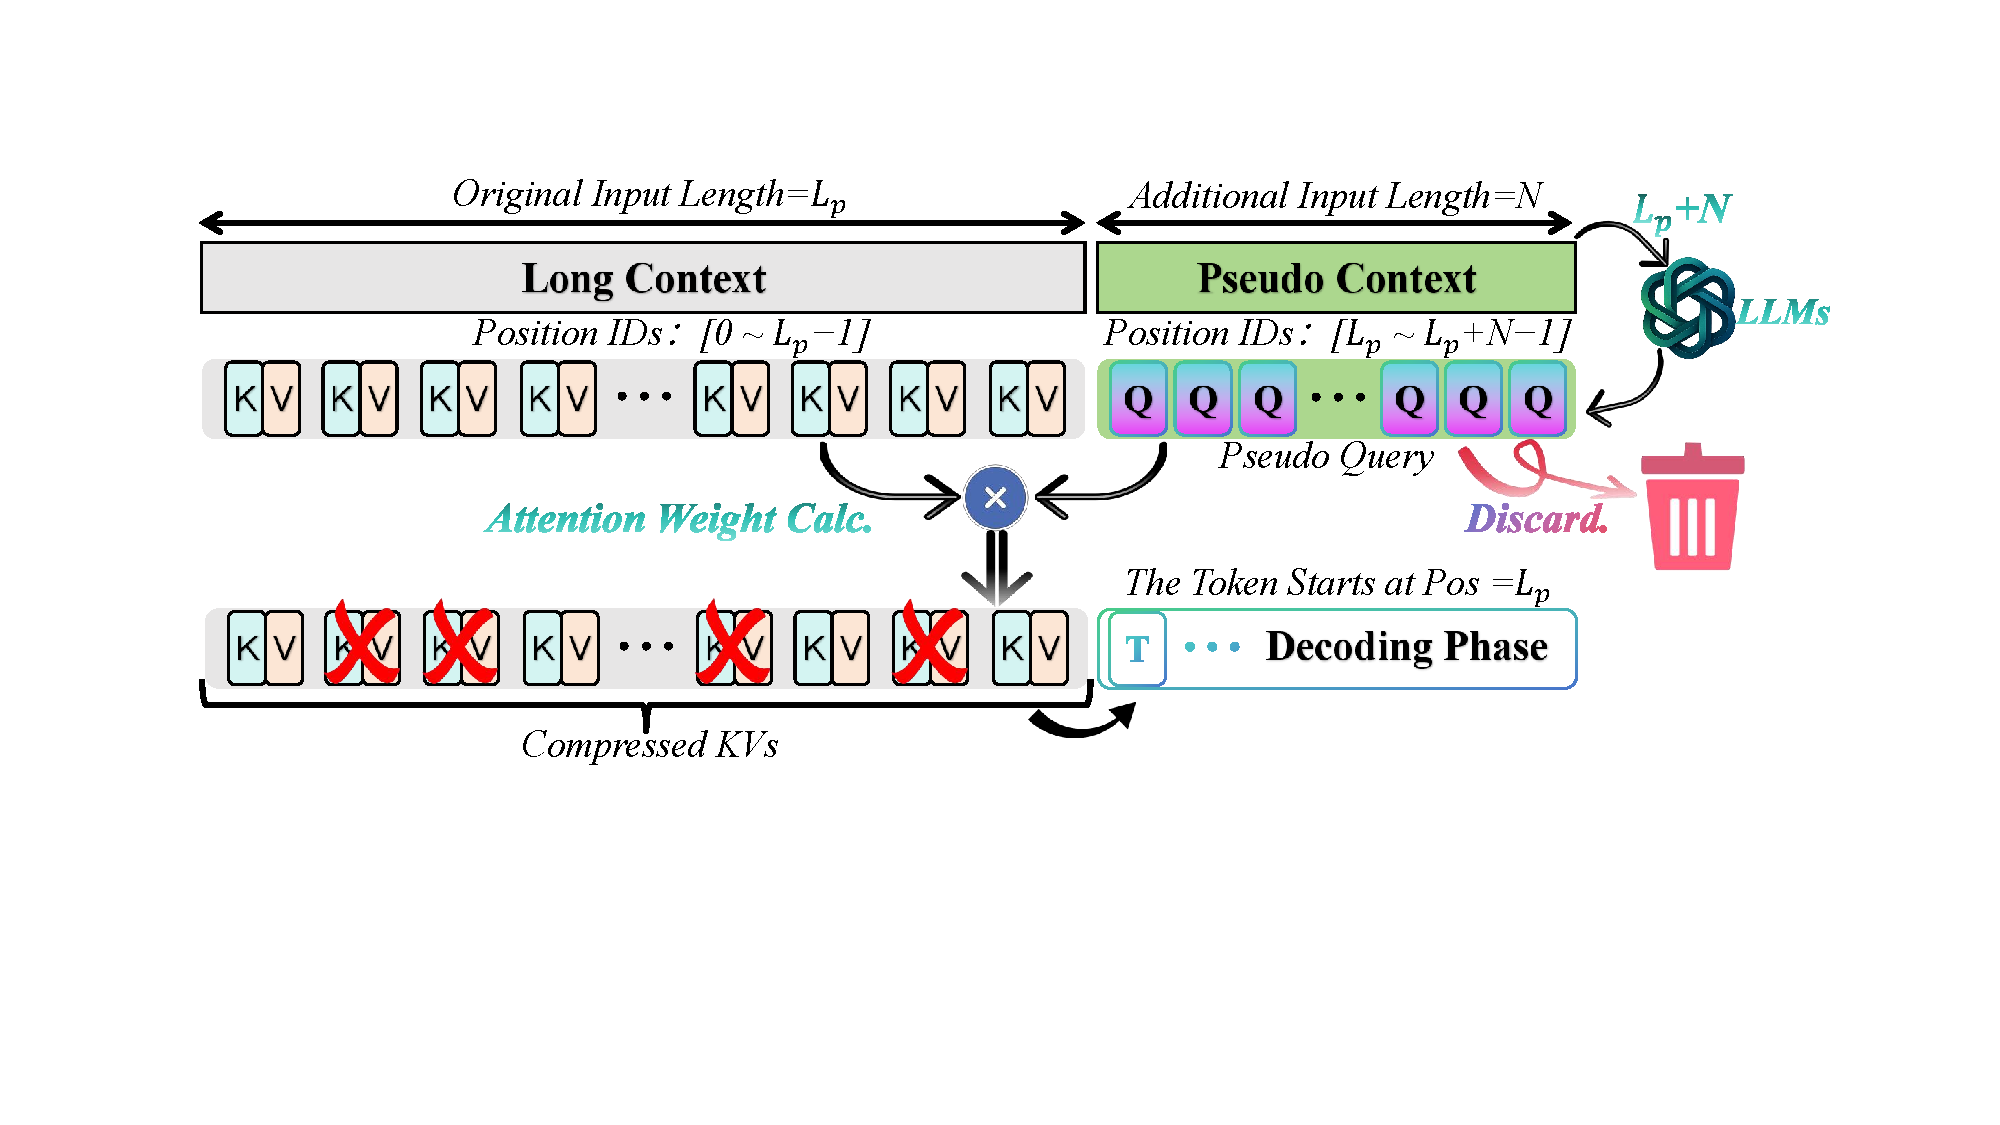
\includegraphics{images/method.pdf}} % 强制调整大小
    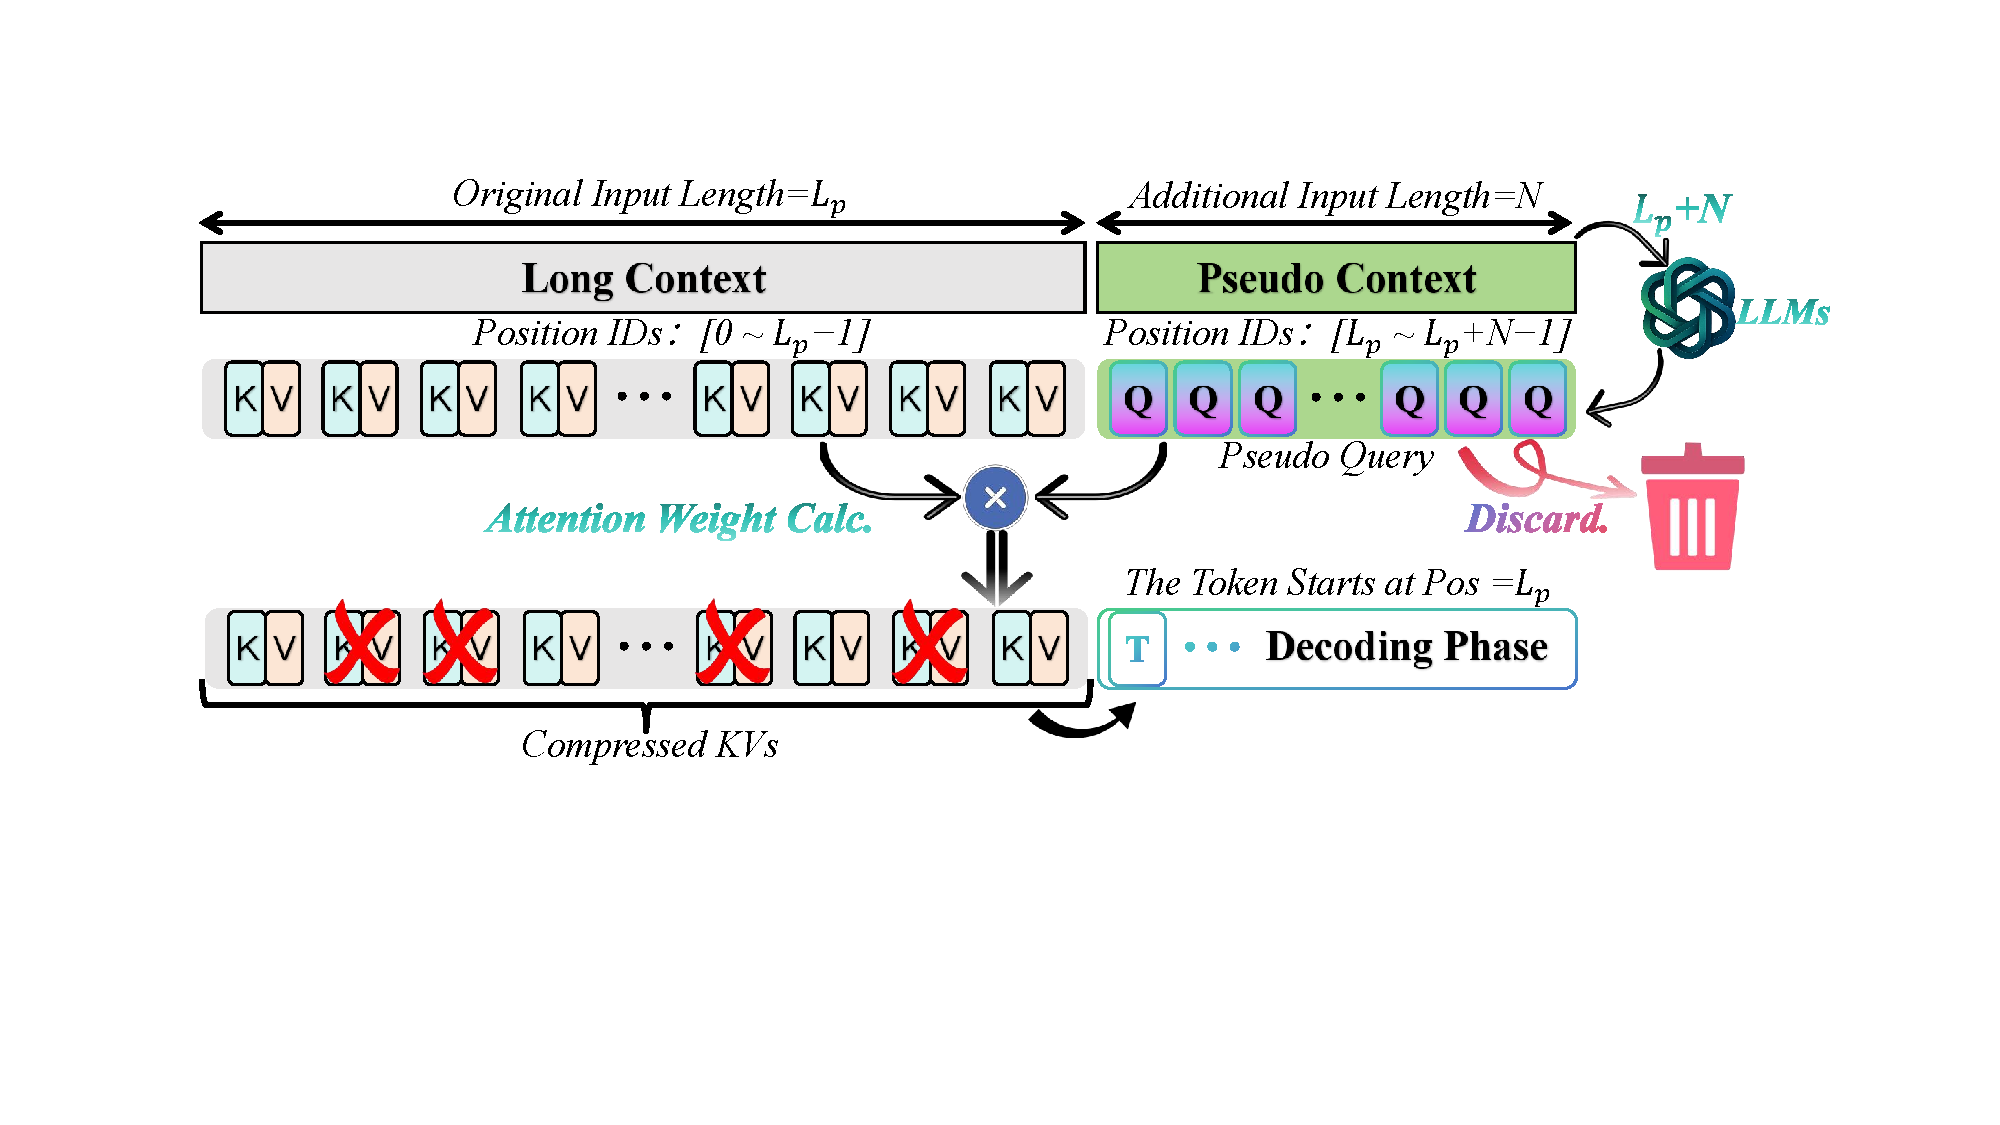
\includegraphics[width=1\linewidth]{images/method.pdf}
    \caption{An overview of DapQ. A synthetic pseudo context (length $N$) is appended to the original context (length $L_p$), forming an extended sequence of length $L_p{+}N$. The model processes this sequence during the prefill phase and then obtains pseudo queries for the synthetic tokens, which are endowed with the correct positional encodings of the first $N$ decoding steps. These pseudo queries compute attention scores with all keys from the original prompt, establishing the token importance distribution. The $topK$ tokens are retained in the compressed KV cache, while the others, along with all the synthetic tokens are evicted. Autoregressive decoding then begins from position $L_p$.}
    \label{fig:DapQ}
    \vspace{-10pt}
\end{figure*}

%当前方法存在的问题、不好的现象
However, the input-centric observation window is inherently misaligned with the dynamic query of actual decoding and relies solely on static prompt-based features, typically the last 16-32 tokens. Consequently, they fail to reflect the importance distribution determined by the output-side generation process, leading to misidentification of the critical tokens for decoding, particularly in complex or noisy contexts. Crucially, ground-truth decoding queries are unavailable during inference, rendering them impractical for directly guiding eviction. To mitigate this, the recent approach LAQ++ \citep{lookahead} attempts to better align the observation window with decoding queries by pre-generating pseudo responses. But its two-stage eviction process introduces a significant memory peak issue that undermines its practical efficiency. Therefore, constructing effective pseudo queries (\texorpdfstring{\(Q_{\text{pseudo}}\)}{Q\_pseudo}) to approximate unavailable future queries without incurring any memory overheads is highly desirable.


%我们发现
Inspired by CaliDrop \citep{calidrop}, where queries at adjacent positions exhibit high similarity, our experiments uncover a pivotal insight: \textbf{positional information plays a more critical role than semantic content in constructing query approximations and determining attention patterns}. This discovery implies that high-quality pseudo queries, capable of reliably assessing the importance distribution of KV cache, can be synthesized based on future positional encodings.

 
%我们提出的method
Motivated by this insight, we propose decoding-aligned KV cache compression via position-aware pseudo queries (\textbf{DapQ}), a novel and lightweight KV cache eviction framework that constructs pseudo queries using future positional encodings to accurately simulate the output tokens. These queries collectively serve as an effective observation window for importance scoring that aligns closely with the actual generation context, enabling precise cache eviction. Extensive experiments across multiple benchmarks and different LLMs demonstrate that DapQ achieves superior performance and outperforms existing eviction baselines, particularly under strict memory constraints. 
% Our work enables high-performance long-context inference, opening a new path for future advancements in LLMs optimization.
% ————————————————————————————————————————————————————————————————
% Moreover, DapQ can be orthogonal to existing strategies, serving as a plug-and-play module that can be seamlessly integrated to achieve further performance gains.
% DapQ's core innovation lies in its ability to effectively simulate decoding behavior solely through precise positional foresight, circumventing the need for expensive content pre-generation and achieving efficient yet accurate cache compression.
% ————————————————————————————————————————————————————————————————
% Contributions. We mainly:
% (1) Uncover the dominance of positional information over semantic content in approximating decoding queries and determining attention patterns.
% (2) Propose DapQ, a novel eviction framework that synthesizes an effective observation window using position-aware pseudo-queries, enabling decoding-aligned compression without pre-generation or extra memory overhead.
% (3) Demonstrate through extensive evaluation that DapQ consistently outperforms existing baselines across diverse models and benchmarks, especially under strict memory constraints.
% ————————————————————————————————————————————————————————————————
% Our contributions are summarized as follows:
% \begin{itemize}[leftmargin=*,noitemsep, topsep=2pt]
% \item{We uncover a fundamental phenomenon that positional information plays a more critical role than contextual content in constructing query approximations and determining attention patterns.}
% \item{We propose DapQ, a novel and lightweight KV cache eviction framework that leverages position-aware pseudo-queries to simulate future decoding contexts. This allows for accurate token importance estimation and cache compression without pre-generation or extra memory overhead.}
% \item{We conduct extensive experiments across five long-context benchmarks and four LLM architectures, showing that DapQ consistently achieves superior performance, particularly under strict memory constraints. } 
% \end{itemize}
\label{sec:introduction}